\documentclass{jsbook}
\usepackage[dvipdfmx]{graphicx}
\usepackage{ascmac}
\begin{document}
\chapter{Paillet6編}
ループを持つ論理回路についてのパートです。\\
自分で学習したものとして詳細な解説は無くして、メモ程度になっています。
部分によっては丁寧に解説しているところもありますが。
\newpage
\section{Paillet6について}
高橋教授の先行研究で中で扱われた回路のうちの1つです。
回路図は図\ref{paillet6}のようになっています。
この回路のモデル化と検証をします。
\begin{figure}[htbp]
\begin{center}
  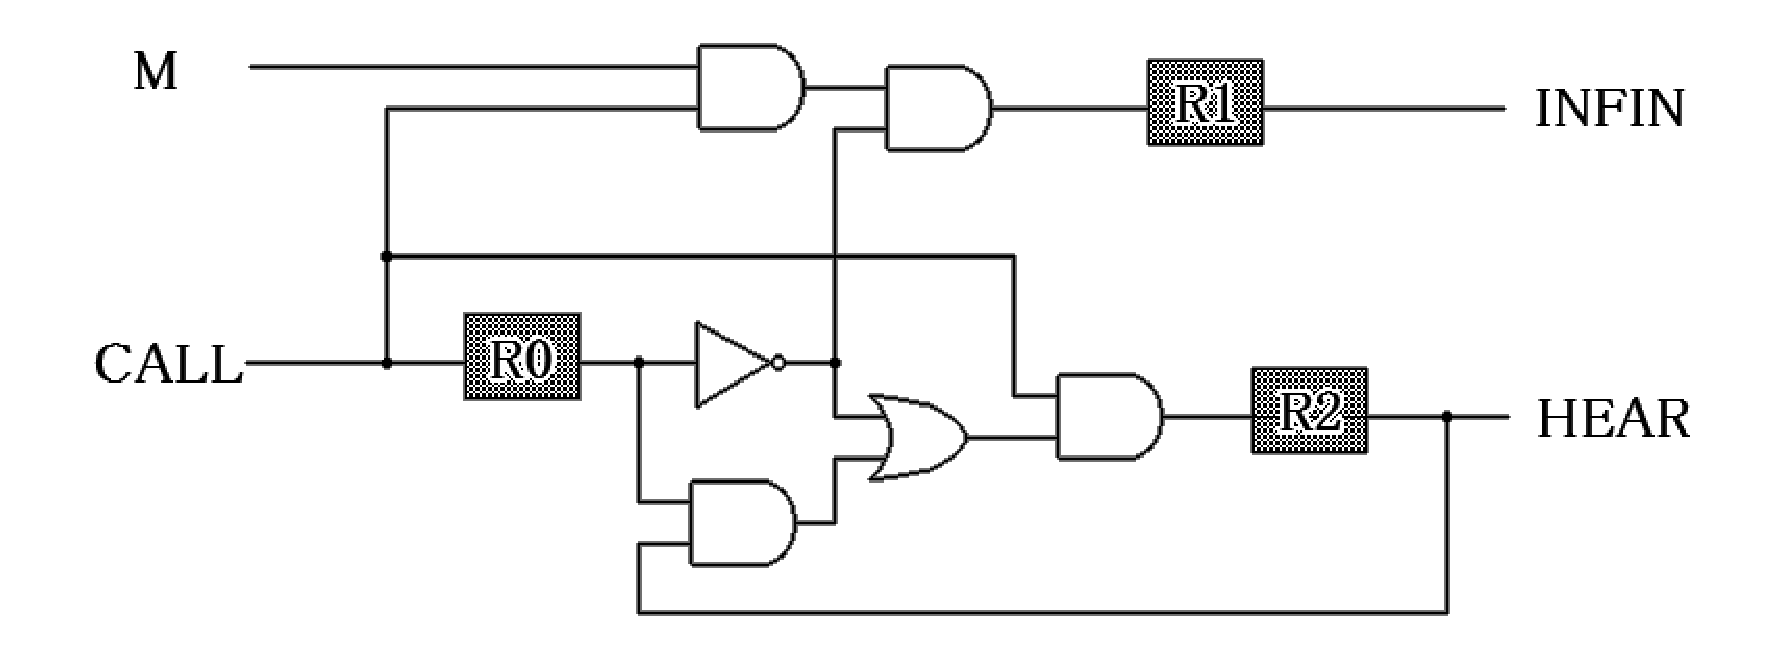
\includegraphics[width=38zw]{image/Paillet6_AE.eps}
  \caption{Paillet6回路}
  \label{paillet6}
\end{center}
\end{figure}

\section{レジスタについて}
加算器と違い、この回路はレジスタを含んでいます。
回路図のR1、R2、R3がそうです。
レジスタには種類がありますが、ここで用いられているレジスタは「入力を1時刻遅らせて出力する」という機能で、いわゆる遅延素子です。
Paillet6の場合は別の実装方法をしていますが、この機能だけを実装したら以下のようになりました。
\begin{verbatim}
Fixpoint delayn(n : nat)(l: list nat): list nat :=
match n with
| 0 => l
| S n' => match l with
          | nil => [0] ++ (delayn n' nil)
          | a::l' => [0] ++ (delayn n' l)
          end
end.
\end{verbatim}
入力の自然数でどれだけ遅延させるかを決め、パターンマッチの中で再帰的に自身を呼び出すことによって複数回遅延を表現しています。
これは自然数 natの場合の遅延ですが、boolの場合でも同様の書き方で定義できます。
変えるべきところは変える必要は当然ありますが。
Paillet6での実装方法はその時に説明します。
\section{Paillet6のモデル化}
基本的には先行研究のモデルを再現するという考えのもと、実装していったのでモデルは先行研究とほぼ同じです。
先行研究ではNQTHMという定理証明器を用いて検証していました。
それをCoq用に書きなおすのが主でした。
しかし、そのままではCoqでは扱えないものがあるので、それは自分で考えながら書き換える必要がありました。

たとえば、natを入力するとboolが出力されるという関数は定義できません。
\begin{verbatim}
Definition test1 (a:nat) : bool := .
\end{verbatim}
と書いた場合は関数の中身を書くことが出来ませんし、
\begin{verbatim}
Definition test2 := nat -> bool.
\end{verbatim}
と書くと、読み込んでくれますが、これを使って別の関数を定義する場合に、型が違うと言われてしまいます。
これ解消するためにDefinitionではなく「Parameter」を使います。
これは関数の中身がかけない代わりに、test2のような書き方で型を合わせることが出来ます。
その代わり、証明モードで展開することが出来ません。
\begin{verbatim}
Parameter test3 = nat -> bool.
\end{verbatim}
と書いて、unfoldしてもnat->boolにはならず、test3のままです。
場合によっては、うまく行かなくなる場合がありますが、今回の場合はかなり内側の、一番展開がされた時にようやく登場するので問題ありません。

\begin{itembox}[l]{Paillet6のモデル}
\begin{verbatim}
Definition tau := nat.
Parameter call : tau -> bool.
Parameter m : tau -> bool.

Definition m1 := nat -> bool .

Definition r0_b := call .
Definition r0_a (t:tau) (s0:bool) : bool :=
match t with
| 0 => s0
| S n => r0_b n
end.

Definition r1_b (t:tau)(s0:bool) : bool :=
andb ( andb (m t) (call t)) (negb (r0_a t s0)).

Definition r1_a (t:tau)(s0 s1 : bool) : bool :=
match t with
|0 => s1
|S n => r1_b n s0
end.

Fixpoint r2_a (t:tau)(s0 s2 : bool) : bool :=
match t with
|0 => s2
|S n => andb (call n) 
       (orb (negb (r0_a n s0)) (andb (r0_a n s0) (r2_a n s0 s2)))
end.

Definition infin (t:tau)(s0 s1 : bool) : bool :=
r1_a t s0 s1.

Definition hear (t:tau)(s0 s2 : bool) : bool :=
r2_a t s0 s2.
\end{verbatim}
\end{itembox}
\section{証明}
\end{document}